\section{Method}
The general idea is to generate the medial axis transform and round the distance measures to integer multiples of the nominal bead width,
so that there is never a gap region left over in the middle of the polygon.

We round to ingteger multiples of half the nozzle width so as to allow single-bead segments.
These could be printed from polygon and return to polygon over same segment without extruding

\begin{figure}
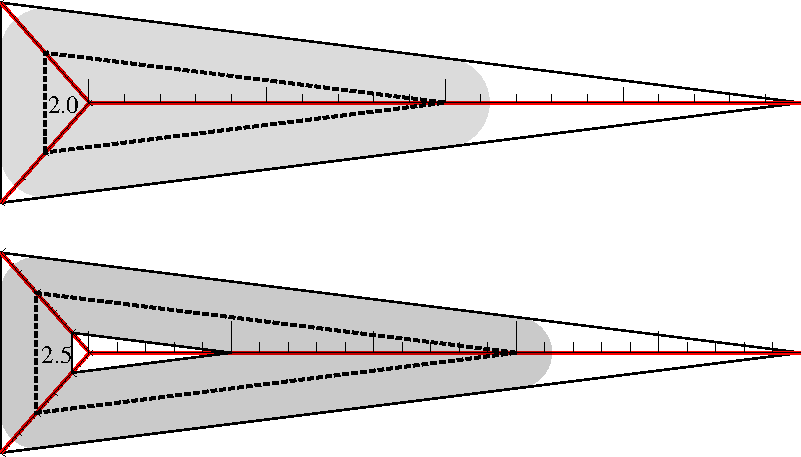
\includegraphics[width=\columnwidth]{sources/method/rounded_vs_unrounded.pdf}
\caption{Toolpaths employing dist rounding vs without.}
\label{rounded_vs_unrounded}
\end{figure}


\begin{figure}
\begin{subfigure}{0.45\columnwidth}
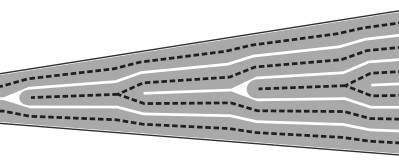
\includegraphics[width=\columnwidth]{sources/method/single_bead_strategy.jpg}
\caption{Overview}
\label{single_bead_strategy_overview}
\end{subfigure}
\begin{subfigure}{0.45\columnwidth}
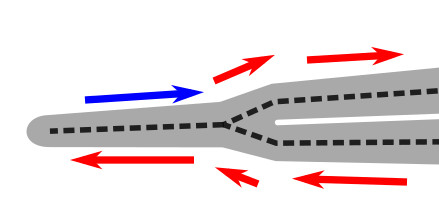
\includegraphics[width=\columnwidth]{sources/method/single_bead_strategy_order.jpg}
\caption{Travel order}
\end{subfigure}
\caption{We can do single-bead segments. Blue is travel move.}
\label{single_bead_strategy}
\end{figure}


\subsection{Overview}
\begin{enumerate}
\item compute medial axis transform (MAT)
\item find places `of high curvature' in the medial axis and mark those regions
\item transform the MAT distance measures in the marked regions to enable fitting an integer multiple beads.
		This transformation uses trasnition regions to smoothly transition from $n$ into $n+1$ insets.
\item introduce extra `joints' on the medial axis in order to discretize the transformed distance measure
\item connect these new joints to the outline with new `bones' (In the standard MAT manner)
\item (optional) transform MAT distance fields along all bones, while keeping the endpoint dist measures fixed. (Deviate from evenly distributed linear space in order to have outer outlines closer to the nominal bead width and only change the innermost couple of toolpaths.)
\item define locations everywhere on the bones of the medial axis at integer MAT distances
\item connect all locations with odd distance measure to form the inset toolpaths
\item connect all even locations to form the extent of the toolpaths, which defines the variable width of the segments.
\end{enumerate}








\subsection{1. Compute MAT}

\begin{figure}
% from /home/t.kuipers/Documents/PhD/Variable_Width_project/pathplanning preliminaries/straight_skeleton_vs_medial_axis.svg
\begin{subfigure}{0.45\columnwidth}
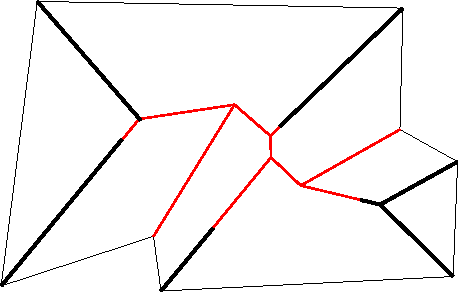
\includegraphics[width=\columnwidth]{sources/method/example_straight_skeleton.pdf}
\caption{Straight skeleton}
\end{subfigure}
\begin{subfigure}{0.45\columnwidth}
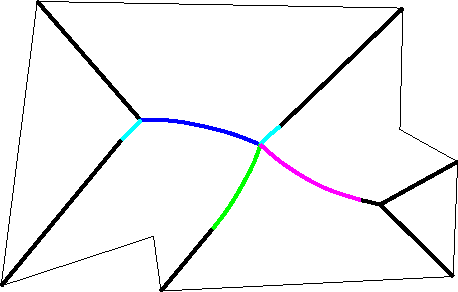
\includegraphics[width=\columnwidth]{sources/method/example_medial_axis.pdf}
\caption{Medial axis}
\end{subfigure}
\caption{Example polygon middle analysis thingies. Difference is colored.}
\label{medial_axis_vs_straight_skeleton}
\end{figure}


\paragraph{Medial axis rather than Straight Skeleton}
See \cref{medial_axis_vs_straight_skeleton}.
Medial axis handles concave corners differently:
instead of generating the bisector, it will generate a parabolic arc in between the vertex and another line segment of the outline polygon.

Medial axis is stable against small perturbations in the input polygon!
Concave corners are handled irrespective of how many vertices are in a corner.


$\to$ approximate parabolas for simpler processing!
A straight skeleton can be made to coincide with the medial axis by changing concave corners into an infinitesimal circle arc;
this does introduce a lot of extra bones, though.






\subsection{2. High curvature marking}
\label{sec:transitioning_cutoff}
\Cref{rounded_dist_measures}
We mark bones as to-be-transformed based on the angle between the two edges of the polygon for which this bone is the bisector.
We generalize this concept of angle to parabola sections and to MAT sections generated by two outline verts.

\paragraph{line-line-segments}
When the angle between two outline segments is small, the naive method will produce long triangular gaps.
We can measure the angle between two outline segments which generate a MAT segment by looking at the angle where the lines going through those segments (would) meet.
Equivalently we can compare the Euclidean distance between two vertices with the difference in distance measure;
if the Euclidean distance is larger than twice the distance measure difference, the angle between the segments is less than {\SI{60}{\degree}}.

\begin{figure}[H]
\centering
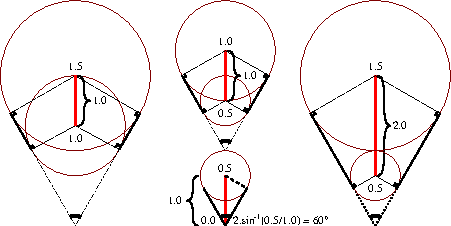
\includegraphics[width=.9\columnwidth]{sources/method/distance_based_angles.pdf}
\caption{Distance based angle estimation. By comparing the euclidean distance between two vertices with the distance measure of the MAT we can skip comparing the angles between the outline segments.}
\label{distance_based_angles}
\end{figure}

The Euclidean distance between two MAT vertices can never be less than the difference in the MAT distance measure between the vertices:t
\begin{figure}[H]
\centering
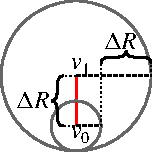
\includegraphics[width=.3\columnwidth]{sources/method/distance_ratio_limit.pdf}
\caption{Minimal Euclidean distance for a given difference in MAT distance measure.}
\label{distance_ratio_limit}
\end{figure}




\paragraph{line-point segments}
For a parabola MAT segment generated by point $(0,d)$ and an outline segment lying on the x-axis, the parabola is given by $y = \frac{1}{2d} x^2 + \frac12 d$.
The angle between the outline segments is twice the angle between the MAT segment and an outline segment.
The angle between the MAT parabola and the x-axis is the inverse tangent of the derivative of this formula: $\tan^{-1} \left( \abs x / d \right)$.
The angle is less than \SI{60}{\degree} when 
$\tan^{-1} \left( \abs x / d \right) < \SI{30}{\degree}$ 
i.e. when $\abs x/d < 1 / \sqrt{3}$
i.e. when $\abs x < d / \sqrt{3}$.
So we mark the part of the parabola as to-be-transformed for which $x \in [-d / \sqrt{3}, d / \sqrt{3}]$.


\paragraph{point-point segments}
For a segment gerenated by points $(0,0)$ and $(0,d)$, the MAT segment is given by $y=\frac12 d$.
For a given $x$ the distance $D$ to the outline vertices is given by $D = \sqrt{x^2 + \frac12 d}$.
The ratio between MAT distance $D$ and Euclidean distance $\abs x$ is determined by $\frac{\partial D}{\partial x} / \frac{\partial \abs x}{x} = \abs \frac{x}{\sqrt{x^2 + d/2}}$
So the Euclidean distance is more than twice the MAT distance then $\abs \frac{\partial D}{\partial x}  < \frac12$, 
%Wolfram Alpha:
so $\abs x < \frac{\sqrt{d}}{\sqrt{6}} \approx 0.408 d$.
So we mark the part of the straight MAT segment as to-be-transformed for which $x \in [-\frac{\sqrt{d}}{\sqrt{6}}, \frac{\sqrt{d}}{\sqrt{6}}]$.
\hl{But that is very weird in combination with the rule that the ends of marked segments should always be rounded! Isn't it?!}








\subsection{3. MAT distance transformation}

\begin{figure}
\centering
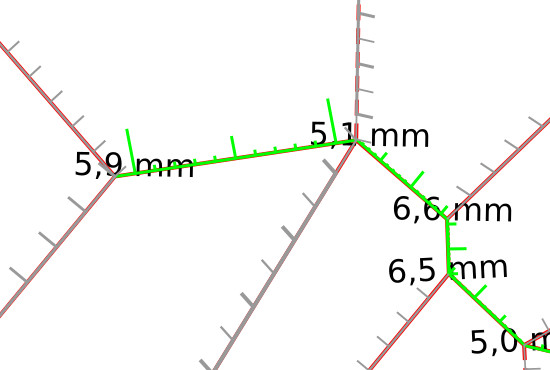
\includegraphics[width=.6\columnwidth]{sources/method/rounded_dist_measures.jpg}
\caption{Distance measure rounding}
\label{rounded_dist_measures}
\end{figure}

See \cref{rounded_dist_measures}.

In a narrow wedge region (a.k.a. a cusp) we have to transfer from $n$ to $n-1$ beads; this transition requires a distance.
See \cref{single_bead_strategy_overview}.
We use a distance of the median bead width for the transition.
The transition needs to be robust against extra fingers in the MAT
How do we compute the vertex location of an inset on a finger which crosses a transitional segment in the middle?

By aligning the MAT distance with Euclidean space around the transition locations, we obtain a stable method for determining the vertex locations of insets.
See \cref{distance_rounding_transition}.
The extra fingers (blue) cause a negligible difference in the inset path (compare the black dashed pat hwith the red dashed path).

\begin{figure}[H]
\centering
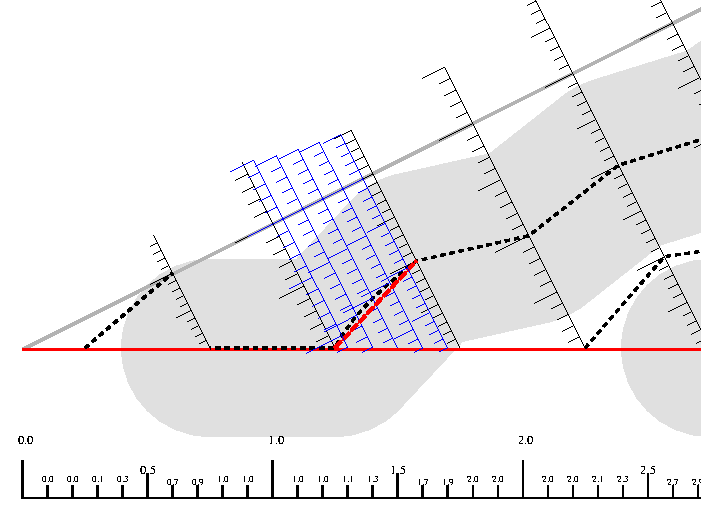
\includegraphics[width=.9\columnwidth]{sources/method/distance_rounding_transition.pdf}
\caption{MAT distance remapping.}
\label{distance_rounding_transition}
\end{figure}



\subsubsection{Ends of markings}
For vertices at the end of a sequence of marked MAT segments we need to perform rounding on the MAT distance measure, so as to avoid a gap being generated by toolapths around that vertex.
See bottom of \cref{rounded_vs_unrounded}.

It impossible for three marked edges to come together.
(Simple case) If 2 edges of the MAT meet then 3 outline segments are involved; lines through those segments form a triangle which cannot have more than two angles less than \SI{60}{\degree}.

However, \hl{what if we connect two marked segments using a small segment?}
It seems there is some distance limit based on \cref{distance_ratio_limit}.






\subsection{4. Introduce joints at key MAT dists}
At the locations where the distance measure changes.
We discretize the distance measure field piecewise linear.
In \cref{distance_rounding_transition} we have one piece at MAT dist $0.0$ from bar $0$ to bar $2.5$, than a piece increasing from MAT dist $0.0$ to $1.0$ from bar $2.5$ to $7.5$ etc.

At the end of a marked section we round the MAT distance measure to the nearest integer and introduce a joint there and connect it to the outline using a new finger.
At those places we round the distance measure without applying transitioning, because the end of the transition would lie beyond the marked region.
 
\paragraph{Note}
We could introduce bones implicitly.
Instead of changing the straight skeleton and introducing bones,
we can simply introduce new vertices on the polygon and generate a new straight skeleton.

\textcolor{gray}{
One could think that this means that the method for introducing joints in the original medial axis should be the same method as used for introducing joints on the newly added fingers connected to the joints introduced in the first step!
}
However, the method for introducing joints on the marked regions may differ from the method for introducing joints on the non-marked regions!









\subsection{5. Add bones for introduced joints}
\textcolor{gray}{
\paragraph{Angle of fingers introduced on the skeleton}
\Cref{finger_angles}
Cannot be optimized.
Always has to be orthogonal to the polygon segment.
Otherwise the algorithm isn't stable w.r.t. extra vertices in the outline.
}
\begin{figure}[H]
\begin{subfigure}{0.45\columnwidth}
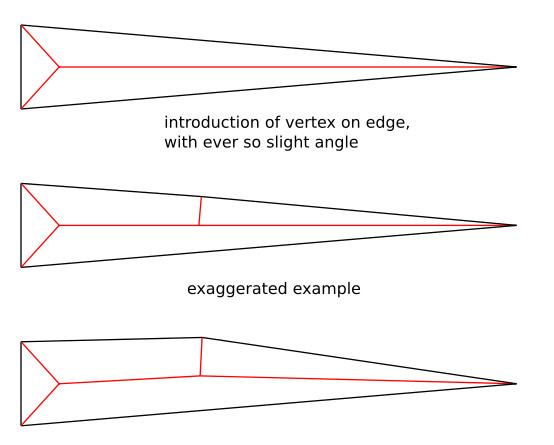
\includegraphics[width=\columnwidth]{sources/method/finger_angles.jpg}
\caption{Stability against extra vertices}
\label{finger_angles_stability}
\end{subfigure}
\begin{subfigure}{0.45\columnwidth}
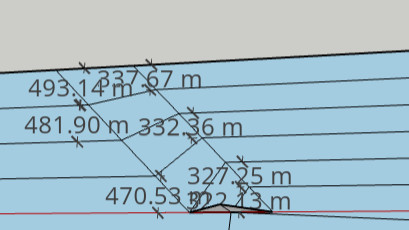
\includegraphics[width=\columnwidth]{sources/method/finger_angles_2.jpg}
\end{subfigure}
\caption{Figner angles should always be orthogonal to the outlines}
\label{finger_angles}
\end{figure}






\subsection{6. transform MAT distance field}
Before generating the locations we can specify a way to space the integer values non-uniformly along a segment.
We can choose have bead widths closer to the nominal bead width near lower MAT dists and do the uniform layout only in the upper region of the segment.
\hl{How do we do this exactly?}

\hl{Is it possible to make this stable against small perturbations?}
See \cref{heterogeneous_joint_generation}.
We must first define a stable end point for where to place the upper region!

\begin{figure}[H]
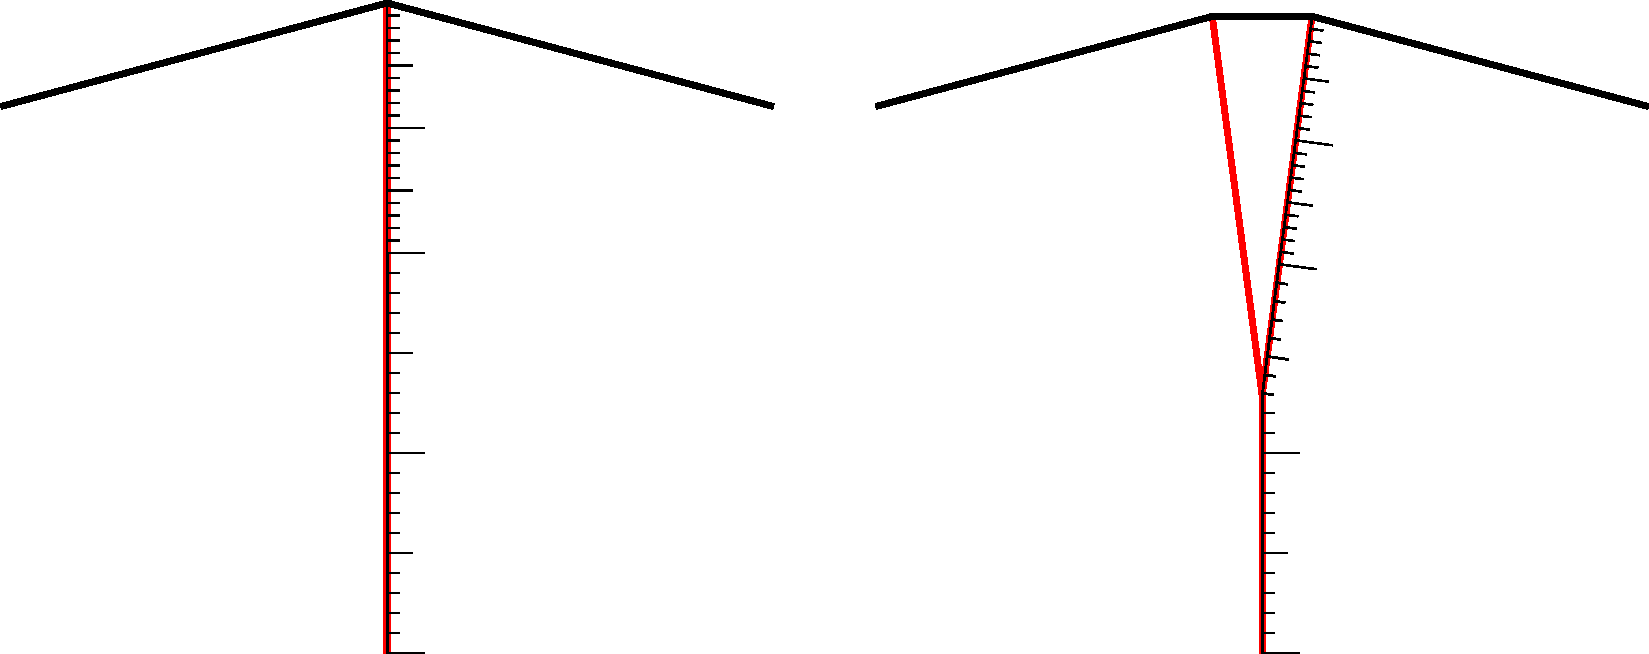
\includegraphics[width=\columnwidth]{sources/method/heterogeneous_joint_generation.pdf}
\caption{Toolpaths employing dist rounding vs without.}
\label{heterogeneous_joint_generation}
\end{figure}






\subsection{7. Location spacing}
\textcolor{gray}{
One could think we should not space the joints evenly along the bones, but make the spacing depend on the angles involved.
We could check the intersection point of the lines of two polygon segments and radially project lines with the same angular spacing.
However, the angular spacing for two patches connected to a single bone would be different, so the paths wouldn't connect!
\hl{Does that mean the angle of the bones should ideally be updated?}
}

\begin{figure}[H]
\centering
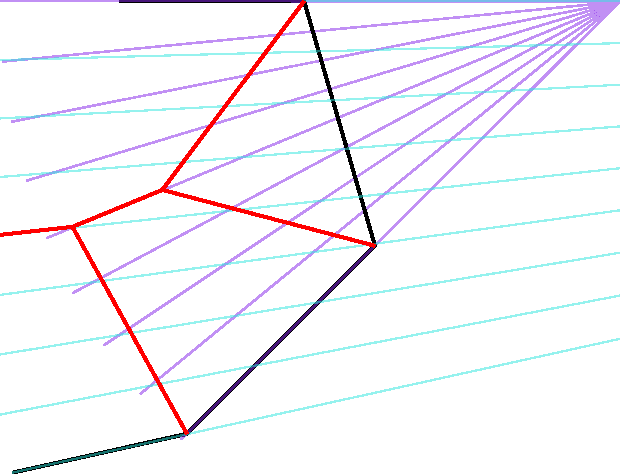
\includegraphics[width=.5\columnwidth]{sources/method/angular_based_spacing.pdf}
\caption{Angular based spacing isn't feasible. The bottom medial axis bone has different spacing based on the two patches. The radially evenly spaced lines are drawn in cyan for the interaction between the bottom outline segment with the top segment and in purple for the interaction between the second bottom segment with  the top segment.}
\label{angular_based_spacing}
\end{figure}


\paragraph{Ideal parabolas}
Subdividing bones introduced for parabolas evenly leads to even spacing along the bone,
while a derived formula seems to produce even spacing in a different sense:
See \cref{medial_axis_parabolas}

\begin{figure}[H]
\begin{subfigure}{0.9\columnwidth}
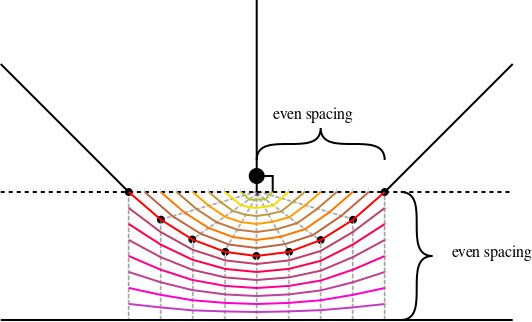
\includegraphics[width=\columnwidth]{sources/method/medial_axis_even_spacing.jpg}
\caption{Parabola transformed to straight skeleton and offsets using even spacing along bones.}
\end{subfigure}
\begin{subfigure}{0.9\columnwidth}
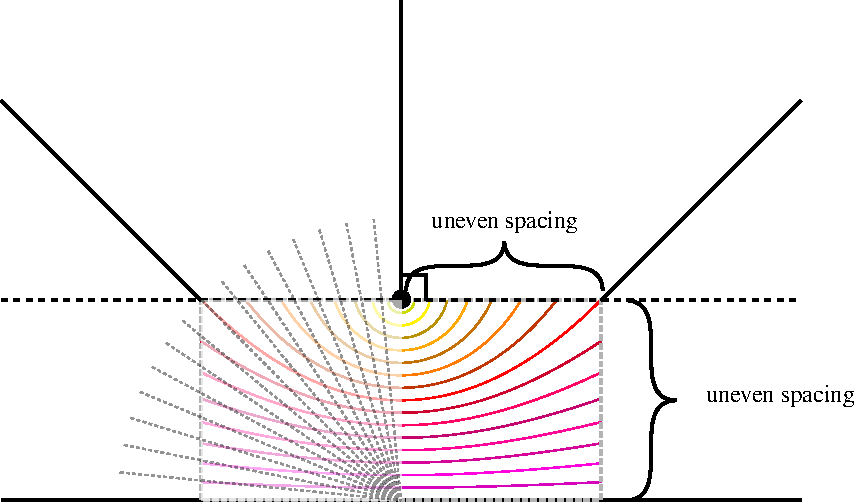
\includegraphics[width=\columnwidth]{sources/method/medial_axis_uneven_spacing.pdf}
\caption{Parabola function plots from analytical solutions where the distance to the point is a whole fraction of the distance to the line.}
\label{medial_axis_parabolas_functions}
\end{subfigure}
\caption{The equidistant points between a vert and a line form a parabola. There are different methods for generating toolpaths which are in between the medial axis and the outline. Note that the uneven spacing does \emph{not} coincide with an even angular spacingat the border between the patches: see the left side of \subref{medial_axis_parabolas_functions}.}
\label{medial_axis_parabolas}
\end{figure}

\hl{But the uneven spacing figure looks like its evenly spaced in the direction orthogonal to the toolpath itself!}






\subsection{8. Connect locations into toolpaths}
\paragraph{Single bead segments}
\Cref{single_bead_strategy}
We round to ingteger multiples of half the nozzle width so as to allow single-bead segments.
These could be printed from polygon and return to polygon over same segment without extruding.
See \cref{single_bead_strategy}.

How to deal with single beads connecting two polys?
: Print 1st poly $\to$ print single bead $\to$ print 2nd poly $\to$ travel over single bead $\to$ print 1st poly

How to deal with three-way intersection single beads?
: Cut up in 1 single bead connecting two polys and 1 normal single bead only connected to one poly






\subsection{Overview}
Below in \cref{parabola_switch_to_less_lines} you can see the different technique preliminaries thought out.
The problem this paper is trying to solve is the large gap in M0.
M1, M2 and M3 use vertices at specific locations and use altered distance measures for those points; these methods are not stable to adding more bones to the skeleton.
M4 and M5 define distance measures in any location (based on \cref{distance_rounding_transition}) which makes them stable.
M5 avoids jagged lines by only applying the MAT distance remapping up to a cutoff point discussed in \cref{sec:transitioning_cutoff}.


\begin{figure*}
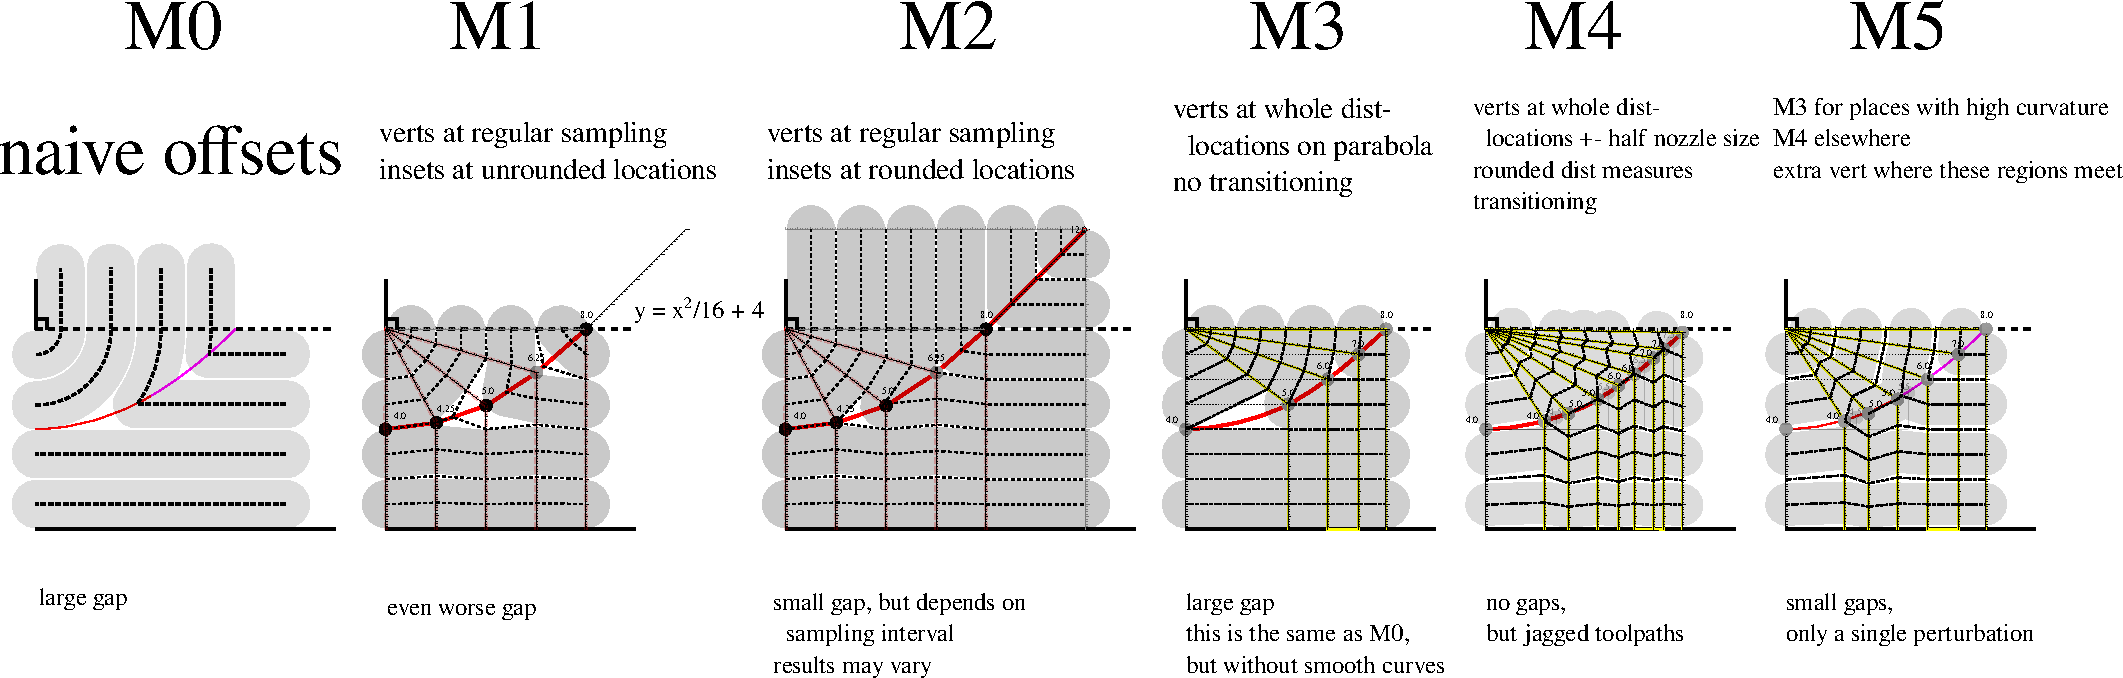
\includegraphics[width=\textwidth]{sources/method/parabola_switch_to_less_lines.pdf}
\caption{Different preliminary variants of the proposed algorithm on a parabola segment.}
\label{parabola_switch_to_less_lines}
\end{figure*}

























































